\documentclass[nooutcomes]{ximera}
\usepackage{booktabs}
%% handout
%% space
%% newpage
%% numbers
%% nooutcomes

\renewcommand{\outcome}[1]{\marginpar{\null\vspace{2ex}\scriptsize\framebox{\parbox{0.75in}{\begin{raggedright}\textbf{P\arabic{problem} Outcome:} #1\end{raggedright}}}}}

\renewenvironment{freeResponse}{
\ifhandout\setbox0\vbox\bgroup\else
\begin{trivlist}\item[\hskip \labelsep\bfseries Solution:\hspace{2ex}]
\fi}
{\ifhandout\egroup\else
\end{trivlist}
\fi}

\newcommand{\RR}{\mathbb R}
\renewcommand{\d}{\,d}
\newcommand{\dd}[2][]{\frac{d #1}{d #2}}
\renewcommand{\l}{\ell}
\newcommand{\ddx}{\frac{d}{dx}}
\everymath{\displaystyle}
\newcommand{\dfn}{\textbf}
\newcommand{\eval}[1]{\bigg[ #1 \bigg]}


\title{Breakout Session 7 Solutions}  

\begin{document}
\begin{abstract}
  % \textbf{A look back:} In the previous (January 28, 2016) Breakout Session you practiced how to interpret and apply the definition of continuity, the intermediate value theorem, and how to determine intervals of continuity.

  % \textbf{Overview:} In today's (February 2, 2016) Breakout Session you will resume the study of rates of change and the relationship between rates of change and graphs of famous functions.

  % \textbf{A look ahead:} In the next (February 4, 2016) Breakout Session you will start to understand the connection between the graph of a derivative and its corresponding (famous) function and discuss the three ways a function is \emph{not} differentiable at a point.
\end{abstract}
\maketitle

% \section{Learning Outcomes}
% \label{section:learning-outcomes}
% The following outcomes are \emph{not an exhaustive} list of the skills you will need to develop and integrate for demonstration on quizzes and exams.
% This list is meant to be a starting point for conversation (with your Lecturer, Breakout Session Instructor, and fellow learners) for organizing your knowledge and monitoring the development of your skills.
% \begin{itemize}
%   \item
%     Use limits to find the slope of the tangent line at a point.

%   \item
%     Write the equation of the tangent line.
    
%   \item
%     Find the derivative function using the limit definition.

%   \item
%     Understand the difference between average and instantaneous velocity.

%   \item
%     Understand secant and tangent lines.

%   \item
%     Understand the definition of the derivative at a point. 

%   \item 
%     Understand the derivative as a function. 
% \end{itemize}

% \newpage
\begin{problem}
  \label{problem:vertical-tangent-line}
  \outcome{Understand secant and tangent lines.}
  \outcome{Understand the definition of the derivative at a point. }
  Define the function $f$ by $f(x) = x^{1/3}$ and consider the graph of this function:
  \begin{image}
    \includegraphics[scale = 0.5]{Images/"Graph for warmup".png}
  \end{image}

  Which of the following two statements are true:
  \begin{itemize}
    \item[(a)]
      The graph of $f$ has a tangent line at $x = 0$.
      \begin{freeResponse}
        This statement is \textbf{true}!
        The function $f$ has a vertical tangent at $x = 0$:
        \begin{image}
          \includegraphics[scale = 0.5]{Images/"Graph with vertical tangent".png}
        \end{image}
      \end{freeResponse}

    \item[(b)]
      The derivative $f'(0)$ is defined.
      \begin{freeResponse}
        This statement is \textbf{false}!
        \begin{align*}
          \lim_{h \to 0^+} \frac{f(0  + h) - f(0)}{h}
          &= \lim_{h \to 0} \frac{h^{1/3}}{h} \\
          \lim_{h \to 0^+} \underbrace{\frac{1}{h^{2/3}}}_\text{form $1/0^+$} &= \infty \\
          &\implies \mbox{$f'(0)$ is undefined}
        \end{align*}
      \end{freeResponse}
  \end{itemize}
\end{problem}

\begin{problem}
  \label{problem:two-different-characterizations}
  \outcome{Understand secant and tangent lines.}
  \outcome{Understand the definition of the derivative at a point.}
    Recall the following two graphs from:
  \[
    \begin{array}{lr}
      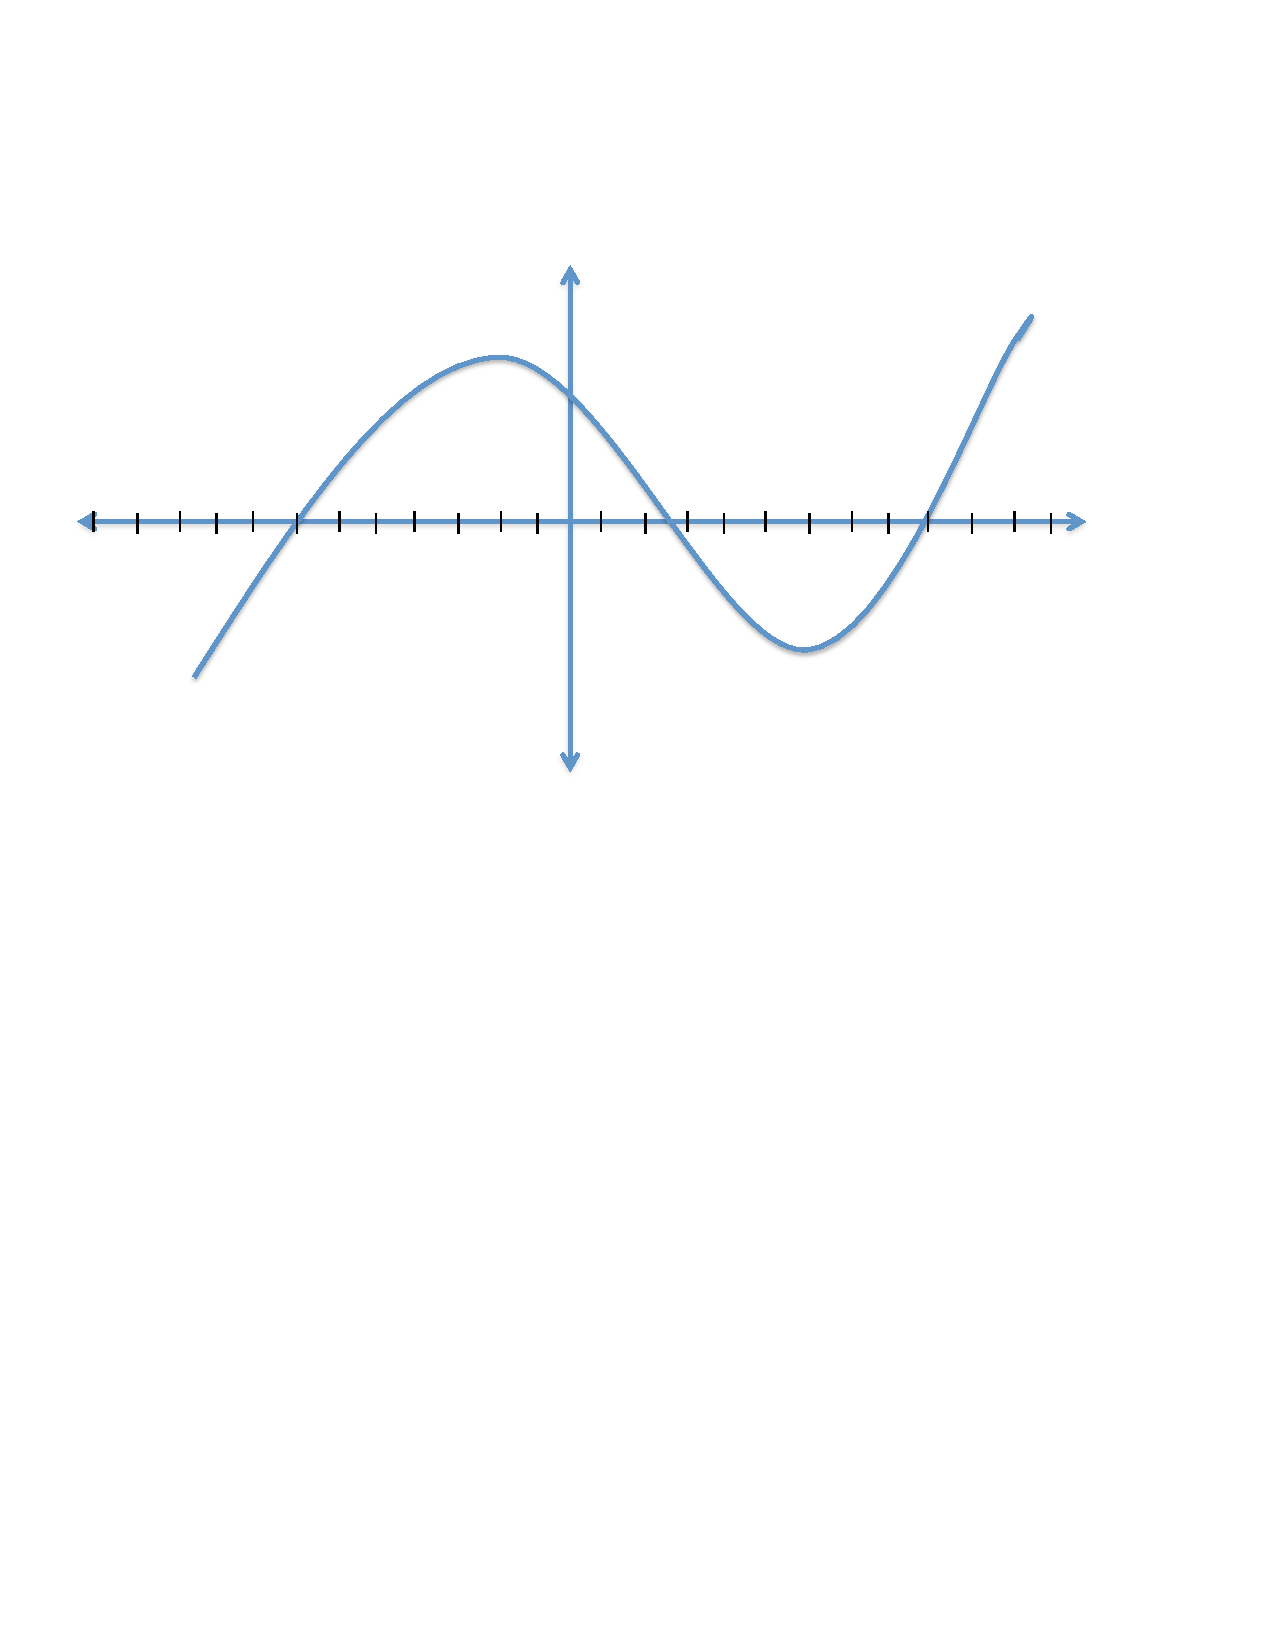
\includegraphics[trim= 150 350 250 180]{Images/Figure2.pdf} &		   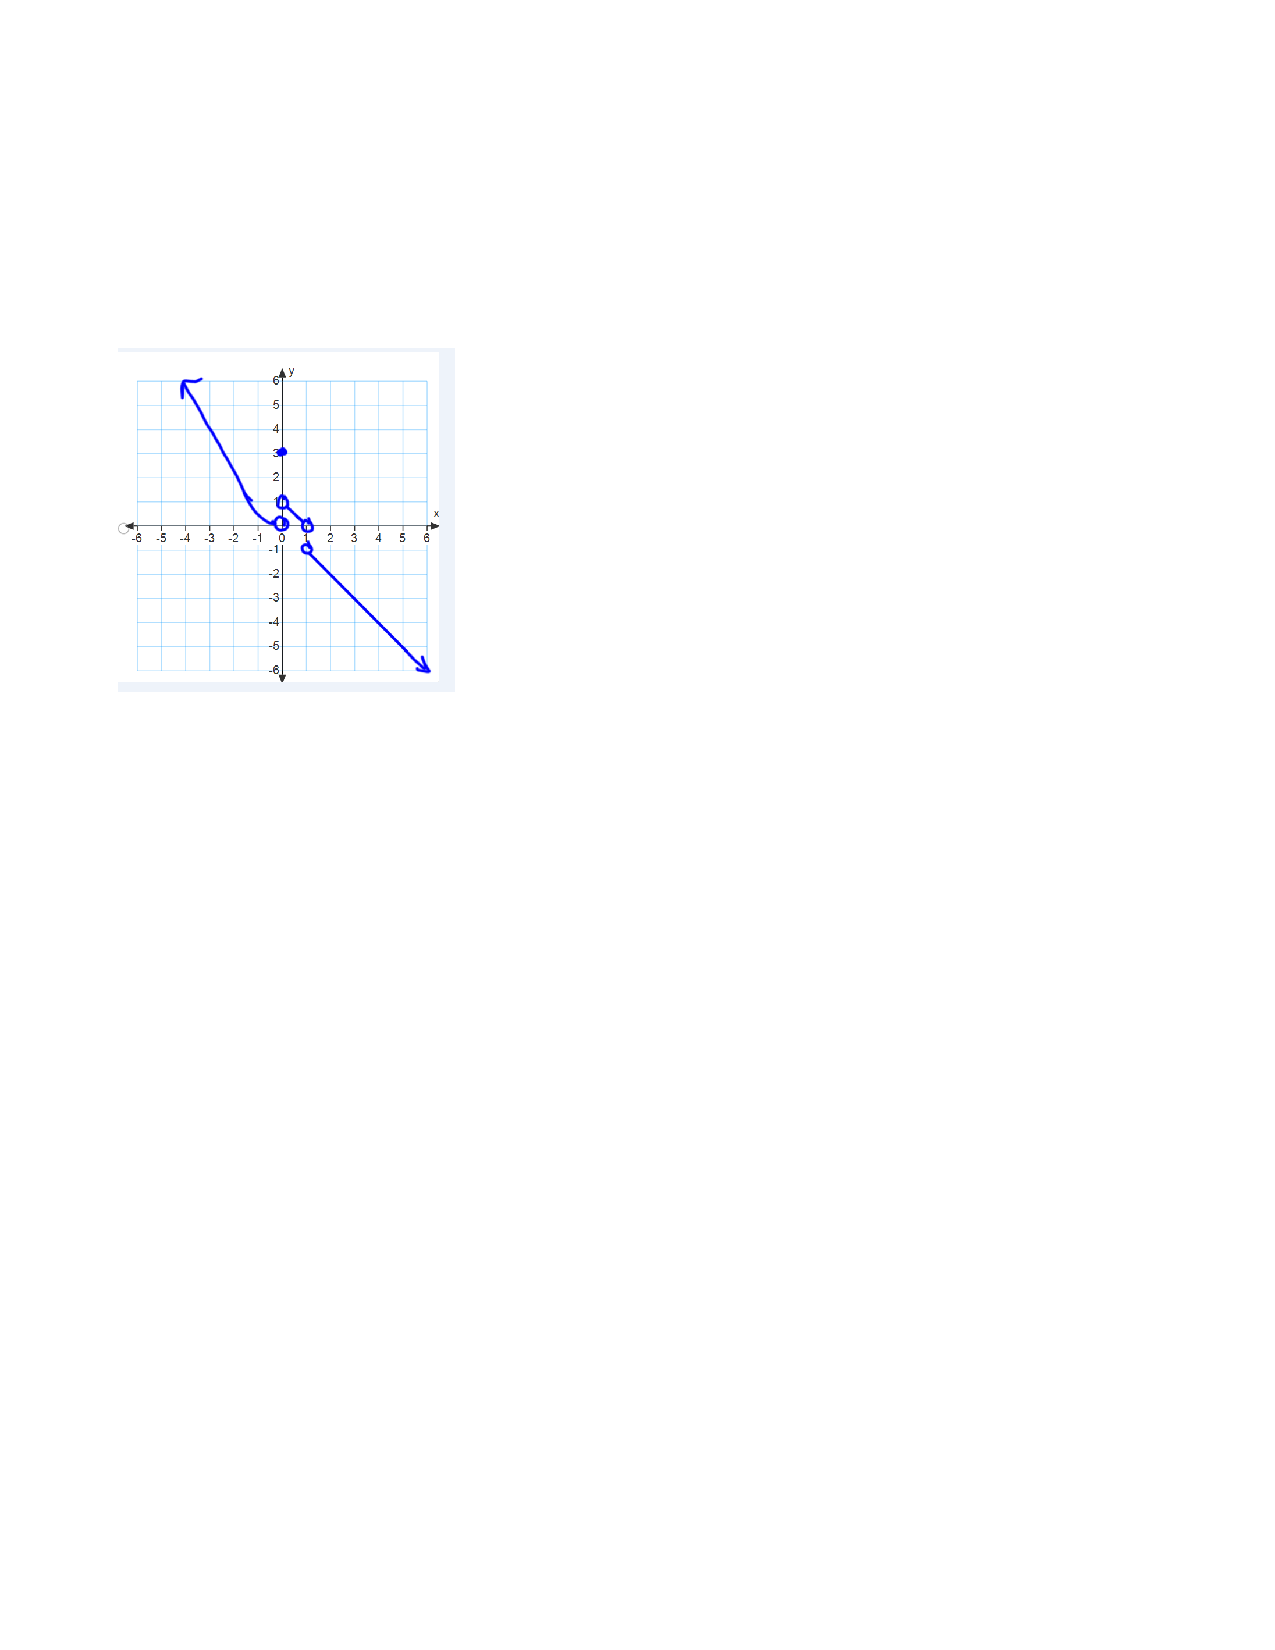
\includegraphics[trim= 140 350 250 180]{Images/Figure3.pdf}
    \end{array}
  \]
  \begin{itemize}
    \item
      What are the similarities between the two graphs?
      \begin{freeResponse}
        The notations 
        \[
          \frac{f(x)-f(a)}{x-a} \quad \text{and} \quad \frac{f(a+h)-f(a)}{h}
        \]
	both express the same number on the two graphs: they each give the slope of the secant line through $P$ and $Q$.

        Also the notations
        \[
          \lim_{x \to a} \frac{f(x)-f(a)}{x-a} \quad \text{and} \quad \lim_{h \to 0} \frac{f(a+h)-f(a)}{h}
        \]
        both express the same number on the two graphs: they each give the slope of the tangent line through $P$.
      \end{freeResponse}

    \item 
      What are the differences?
      \begin{freeResponse}
        Each graph expresses the difference between the $y$-values and $x$-values using two different notations.
        The first graph expresses the difference in a straightforward way---by subtracting the ``first term'' from the ``last term''.
        The second graph expresses the difference in a ``parameterized way''---$h$ plays the role of our ``parameter''.
      \end{freeResponse}

    \item 
      Why is one notation different from the other notation in the graphs?
      \begin{freeResponse}
        Both notations are mathematically equivalent but in a given problem one may be easier to work with than the other.
      \end{freeResponse}

    \item 
      For each of the two graphs, which lines are the secant lines?
      \begin{freeResponse}
        The green line is the secant line in each of the two graphs.        
      \end{freeResponse}

    \item 
      For each of the two graphs, which lines are the tangent lines?
      \begin{freeResponse}
        The red line is the tangent line in each of the two graphs.        
      \end{freeResponse}

    \item 
      What is the main concept these graphs are trying to communicate?
      \begin{freeResponse}
        Both graphs show that as we let $Q$ get closer to $P$, the secant line through $PQ$ approaches the tangent line through $P$.
        We can summarize this by a suggestive phrase: the limit of the secant lines is the tangent line (it is suggestive but not precise).
        Thus the limit of the slopes of the secant lines is the slope of the tangent line.
      \end{freeResponse}
  \end{itemize}
\end{problem}

\begin{problem}
  \label{problem:find-equation-of-tangent-line}
  \outcome{Find the derivative function using the limit definition.}
  \outcome{Use limits to find the slope of the tangent line at a point.}
  \outcome{Understand the definition of the derivative at a point}
  \outcome{Write the equation of the tangent line.}
    For each of the following functions find the equation of the tangent line at the given point.
  \begin{itemize}
    \item[(a)]
      $h(x) = -5x^2 + 7x - 9$ at $x = 3$.
      \begin{freeResponse}
        Slope of tangent line:
        \begin{align*}
          m_{\mathrm{tan}} = \lim_{x \to 3} \frac{h(x) - h(3)}{x-3}
		&= \lim_{x \to 3} \frac{(-5x^2 + 7x - 9) - (-45 + 21 - 9)}{x-3}  \\
		&= \lim_{x \to 3} \frac{-5x^2 + 7x - 9 + 33}{x-3}  \\
		&= \lim_{x \to 3} \frac{-5x^2 + 7x + 24}{x-3}  \\
		&= \lim_{x \to 3} \frac{(x-3)(-5x -8)}{x-3}  \\
		&= \lim_{x \to 3} (-5x - 8)  \\
		&= -5(3) - 8 = -23.
	\end{align*}
        
        Point on tangent line: $(3, h(3)) = (3, -33)$.

        Equation of tangent line:
        \begin{align*}
          y - h(3) = -23(x-3) &\implies y + 33 = -23x + 69\\
          &\implies y = -23x + 36.
        \end{align*}
      \end{freeResponse}

    \item[(b)]
      $g(u) = \sqrt{5u-4}$ at $u = 3$.
      \begin{freeResponse}
        Slope of tangent line:
        \begin{align*}
          m_{\mathrm{tan}} = \lim_{h \to 0} \frac{g(3+h) - g(3)}{h}
            &= \lim_{h \to 0} \frac{\sqrt{5(3+h) - 4} - \sqrt{11}}{h}\\
          \lim_{h \to 0} \frac{\sqrt{5(3+h) - 4} - \sqrt{11}}{h} \cdot \frac{\sqrt{5(3+h) - 4} + \sqrt{11}}{\sqrt{5(3+h) - 4} + \sqrt{11}} \\
		&= \lim_{h \to 0} \frac{5(3+h) - 4 - 11}{h \left( \sqrt{5(3+h) - 4} + \sqrt{11} \right) }  \\
		&= \lim_{h \to 0} \frac{5h + 15 - 15}{h \left( \sqrt{5(3+h) - 4} + \sqrt{11} \right) }  \\
		&= \lim_{h \to 0} \frac{5}{\left( \sqrt{5(3+h) - 4} + \sqrt{11} \right) }  \\
		&= \frac{5}{\sqrt{5(3+0) - 4} + \sqrt{11}}  \\
		&= \frac{5}{2 \sqrt{11}}.
        \end{align*}

        Point on tangent line: $(3, g(3)) = (3, \sqrt{11})$.

        Equation of tangent line:
        \begin{align*}
          y - g(3) = \frac{5}{2\sqrt{11}}(u-3)
          &\implies y - \sqrt{11} = \frac{5}{2\sqrt{11}}(u - 3)\\
          &\implies y = \frac{5}{2\sqrt{11}}u - \frac{15}{2\sqrt{11}} + \sqrt{11}.
        \end{align*}
      \end{freeResponse}

    \item[(c)]
      $\displaystyle s(z) = \frac{z}{z-5}$ at $z = 3$.
      \begin{freeResponse}
        Slope of tangent line:
        \begin{align*}
          m_{\mathrm{tan}}
          &= \lim_{z \to 3} \frac{s(z) - s(3)}{z-3}  \\
		&= \lim_{z \to 3} \frac{\frac{z}{z-5} - \frac{3}{3-5}}{z-3}  \\
		&= \lim_{z \to 3} \frac{\frac{z}{z-5} + \frac{3}{2}}{z-3}  \\
		&= \lim_{z \to 3} \frac{\frac{2z}{2(z-5)} + \frac{3(z-5)}{2(z-5)}}{z-3}  \\
		&= \lim_{z \to 3} \frac{\frac{2z + 3z - 15}{2(z-5)}}{z-3}  \\
		&= \lim_{z \to 3} \frac{5z-15}{2(z-5)} \cdot \frac{1}{z-3}  \\
		&= \lim_{z \to 3} \frac{5(z-3)}{2(z-5)} \cdot \frac{1}{z-3}  \\
		&= \lim_{z \to 3} \frac{5}{2(z-5)}  \\
		&= \frac{5}{2(3-5)} = -\frac{5}{4}.
	\end{align*}

        Point on tangent line: $(3, s(3)) = (3, -3/2)$.

        Equation of tangent line:
        \begin{align*}
          y - s(3) = - \frac{5}{4}(z-3) &\implies y + \frac{3}{2} = - \frac{5}{4}z + \frac{15}{4}\\
          &\implies y = - \frac{5}{4} z + \frac{9}{4}.
        \end{align*}
      \end{freeResponse}
  \end{itemize}
\end{problem}

\begin{problem}
  \label{problem:nondifferentiable-at-point}
  \outcome{Understand the definition of the derivative at a point.}
  \outcome{Find the derivative function using the limit definition.}
   Define the function $f$ by $f(x) = |5-x|$.
  \begin{itemize}
    \item[(a)]
      Find $f'(5)$.
      \begin{freeResponse}
        Check right-sided limit and left-sided limit to determine if $f'(5)$ exists.

        Evaluation of right-sided limit:
        \begin{align*}
          \lim_{x \to 5^+} \frac{|5-x|}{x - 5}
          &= \lim_{x \to 5^+} \frac{-(5-x)}{x - 5} \\
          &= \lim_{x \to 5^+} \frac{x-5}{x - 5}\\
          &= \lim_{x \to 5^+} 1 = 1.
        \end{align*}

        Evaluation of left-sided limit:
        \begin{align*}
          \lim_{x \to 5^-} \frac{|5-x|}{x - 5}
          &= \lim_{x \to 5^-} \frac{5-x}{x - 5} \\
          &= \lim_{x \to 5^+} \frac{-(x-5)}{x - 5}\\
          &= \lim_{x \to 5^+} -1 = -1.
        \end{align*}

        So $f'(5)$ is undefined.
      \end{freeResponse}


    \item[(b)]
      For $a < 5$, find $f'(a)$.
      \begin{freeResponse}
        \begin{align*}
          \lim_{x \to a} \frac{|5-x| - |5-a|}{x - a}
          &= \lim_{x \to a} \frac{|5-x| - (5-a)}{x - a} \\
          &= \lim_{x \to a} \frac{(5-x) - (5-a)}{x - a} \\
          &= \lim_{x \to a} \frac{-(x-a)}{x-a}  \\
          &= \lim_{x \to a} -1 = -1\\
          &\implies \mbox{$f'(a) = -1$ for all $a < 5$}
        \end{align*}
      \end{freeResponse}

    \item[(c)]
      For $a > 5$, find $f'(a)$.
      \begin{freeResponse}
        \begin{align*}
          \lim_{x \to a} \frac{|5-x| - |5-a|}{x - a}
          &= \lim_{x \to a} \frac{|5-x| + (5-a)}{x - a} \\
          &= \lim_{x \to a} \frac{-(5-x) - (5-a)}{x - a} \\
          &= \lim_{x \to a} \frac{(x-a)}{x-a}  \\
          &= \lim_{x \to a} 1 = 1\\
          &\implies \mbox{$f'(a) = 1$ for all $a > 5$}
        \end{align*}
      \end{freeResponse}

  \end{itemize}

\end{problem}
\end{document} 
